\documentclass{article}
\usepackage{tikz}
\usetikzlibrary{decorations.pathmorphing}

\begin{document}

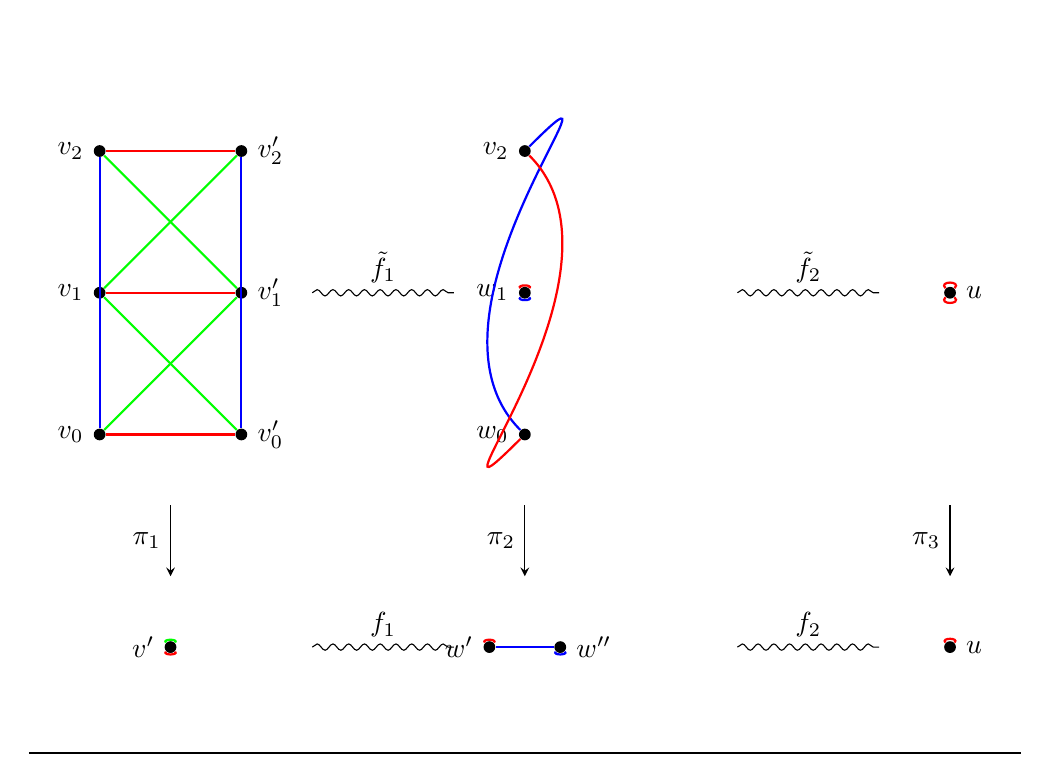
\begin{tikzpicture}[scale=0.9]
% Define styles
\tikzset{
    vertex/.style={circle, fill=black, inner sep=1.5pt},
    wavy/.style={decorate, decoration={snake, amplitude=.4mm, segment length=2mm}}
}

% First graph (top left)
\node[vertex, label=left:$v_2$] (v2) at (0,2) {};
\node[vertex, label=left:$v_1$] (v1) at (0,0) {};
\node[vertex, label=left:$v_0$] (v0) at (0,-2) {};

\node[vertex, label=right:$v'_2$] (v2p) at (2,2) {};
\node[vertex, label=right:$v'_1$] (v1p) at (2,0) {};
\node[vertex, label=right:$v'_0$] (v0p) at (2,-2) {};

% Edges of first graph
\draw[blue, thick] (v2) -- (v0);
\draw[blue, thick] (v2p) -- (v0p);
\draw[green, thick] (v2) -- (v1p);
\draw[green, thick] (v1) -- (v2p);
\draw[green, thick] (v0) -- (v1p);
\draw[green, thick] (v1) -- (v0p);
\draw[red, thick] (v2) -- (v2p);
\draw[red, thick] (v1) -- (v1p);
\draw[red, thick] (v0) -- (v0p);

% Second graph (top middle)
\node[vertex, label=left:$v_2$] (w2) at (6,2) {};
\node[vertex, label=left:$w_1$] (w1) at (6,0) {};
\node[vertex, label=left:$w_0$] (w0) at (6,-2) {};

% Edges of second graph
\draw[blue, thick] (w2) to[out=45, in=135, looseness=1.5] (w0);
\draw[red, thick] (w2) to[out=315, in=225, looseness=1.5] (w0);
\draw[red, thick] (w1) to[out=45, in=135, looseness=1.5] (w1);
\draw[blue, thick] (w1) to[out=315, in=225, looseness=1.5] (w1);

% Third graph (top right)
\node[vertex, label=right:$u$] (u) at (12,0) {};

% Edges of third graph
\draw[red, thick] (u) to[out=45, in=135, looseness=3] (u);
\draw[red, thick] (u) to[out=315, in=225, looseness=3] (u);
\draw[red, thick] (u) to[out=180, in=180, looseness=3] (u);

% Wavy arrows (top row)
\draw[wavy] (3,0) -- node[above] {$\tilde{f}_1$} (5,0);
\draw[wavy] (9,0) -- node[above] {$\tilde{f}_2$} (11,0);

% Vertical arrows
\draw[-stealth] (1,-3) -- node[left] {$\pi_1$} (1,-4);
\draw[-stealth] (6,-3) -- node[left] {$\pi_2$} (6,-4);
\draw[-stealth] (12,-3) -- node[left] {$\pi_3$} (12,-4);

% First graph (bottom left)
\node[vertex, label=left:$v'$] (vp) at (1,-5) {};

% Edges of first bottom graph
\draw[green, thick] (vp) to[out=135, in=45, looseness=1.5] (vp);
\draw[red, thick] (vp) to[out=315, in=225, looseness=1.5] (vp);

% Second graph (bottom middle)
\node[vertex, label=left:$w'$] (wp) at (5.5,-5) {};
\node[vertex, label=right:$w''$] (wpp) at (6.5,-5) {};

% Edges of second bottom graph
\draw[red, thick] (wp) to[out=135, in=45, looseness=1.5] (wp);
\draw[blue, thick] (wp) -- (wpp);
\draw[blue, thick] (wpp) to[out=315, in=225, looseness=1.5] (wpp);

% Third graph (bottom right)
\node[vertex, label=right:$u$] (ub) at (12,-5) {};

% Edges of third bottom graph
\draw[red, thick] (ub) to[out=45, in=135, looseness=2] (ub);

% Wavy arrows (bottom row)
\draw[wavy] (3,-5) -- node[above] {$f_1$} (5,-5);
\draw[wavy] (9,-5) -- node[above] {$f_2$} (11,-5);

% Horizontal line at the bottom
\draw[thick] (-1,-6.5) -- (13,-6.5);

\end{tikzpicture}

\end{document}